\documentclass{../../../oss-classkick-exam}
\usetikzlibrary{decorations.pathmorphing,patterns}

\begin{document}
\genheader

\gentitle{C}{MOMENTUM AND CENTER OF MASS}

\genmultidirections

\gengravity

\raggedcolumns
\begin{multicols*}{2}
  \begin{questions}

%    \question A toy train car of mass \SI{3}{\kilo\gram} rolls to the left at
%    \SI{2}{\metre\per\second} and collides with a \SI{4}{\kilo\gram} train
%    car rolling to the right at \SI{1}{\metre\per\second}. The two cars stick
%    together. The velocity of the cars after the collision is
%    \begin{choices}
%      \choice $2/7$ \si{\metre\per\second} to the left
%      \choice $2/7$ \si{\metre\per\second} to the right
%      \choice $4/7$ \si{\metre\per\second} to the left
%      \choice $4/7$ \si{\metre\per\second} to the right
%      \choice $9/7$ \si{\metre\per\second} to the right
%    \end{choices}
%    \vspace{.7in}
%    
%    \question Two steel balls, one of mass $m$ and the other of mass $2m$,
%    collide and rebound in a perfectly elastic collision. Which of the
%    following is conserved in this elastic collision?
%    \begin{choices}
%      \choice velocity only
%      \choice momentum only
%      \choice momentum and kinetic energy only
%      \choice momentum, velocity, and kinetic energy
%      \choice kinetic energy only
%    \end{choices}
%    \vspace{.67in}

    \question A uniform rod of length $2\ell$ is bent, as shown in the figure
    below. What are the coordinates of the center of mass of the rod?
    \begin{center}
      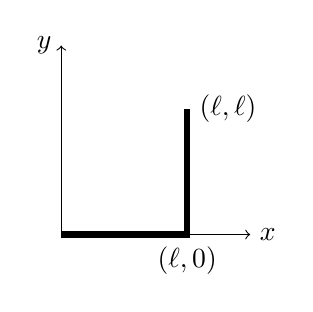
\begin{tikzpicture}[scale=.8]
        \draw[->](0,0)--(3,0) node[right]{$x$};
        \draw[->](0,0)--(0,3) node[left]{$y$};
        \draw[line width=.8mm](0,0)--(2,0) node[below]{$(\ell,0)$}
        --(2,2) node[right]{$(\ell,\ell)$};
      \end{tikzpicture}
    \end{center}
    \begin{choices}
      \choice $(\ell/4,3\ell/4)$
      \correctchoice $(3\ell/4,\ell/4)$
      \choice $(2\ell/3,\ell/3)$
      \choice $(2\ell/3,2\ell/3)$
      \choice $(\ell/2,\ell/3)$
    \end{choices}

    \question Two uniform spheres of masss $M$ and $4M$ are connected by a rod
    whose mass is negligible, and the distance between the centers of the
    spheres is $d$. The $4M$ sphere is then moved a distance of $d/3$ toward the
    smaller sphere. How far has the center of mass of the entire object moved?
    \begin{choices}
      \choice The center of mass has not moved, because both spheres still have
      their original masses.
      \choice $d/15$
      \choice $d/5$
      \correctchoice $4d/15$
      \choice $8d/15$
    \end{choices}
     
    \question A rubber ball of mass $m$ strikes a wall with a speed $\varv$ at
    an angle $\theta$ below the normal line and rebounds from the wall at the
    same speed and angle above the normal line as shown. The magnitude of the
    change in momentum of the ball is
    \begin{center}
      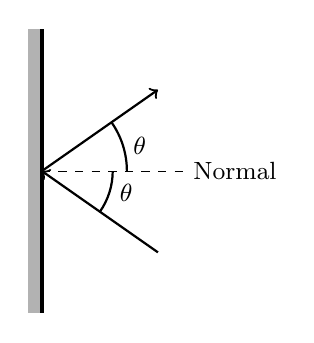
\begin{tikzpicture}[scale=.9]
        \fill[gray!60](-.2,2) rectangle(0,-2);
        \draw[very thick](0,-2)--(0,2);
        \draw[dashed](0,0)--(2,0) node[right]{\small Normal};
        \draw[->,rotate=35, thick](0,0)--(2,0) node[right]{$\varv$};
        \draw[<-,rotate=-35,thick](0,0)--(2,0) node[right]{$\varv$};
        \draw[thick](1,0)  arc(0:-35:1)  node[midway,right]{\small$\theta$};
        \draw[thick](1.2,0)arc(0: 35:1.2)node[midway,right]{\small$\theta$};
      \end{tikzpicture}
    \end{center}
    \begin{choices}
      \choice $mv$
      \choice $2mv$
      \choice $mv\cos\theta$
      \choice $2mv\cos\theta$
      \choice  zero
    \end{choices}
    
    \question Two blocks are connected by a compressed spring and rest on a
    frictionless surface. The blocks are released from rest and pushed apart
    by the compressed spring. If one mass is twice the mass of the other,
    which of the following is the same for both blocks?
    \begin{choices}
      \choice magnitude of momentum
      \choice acceleration
      \choice speed
      \choice kinetic energy
      \choice potential energy
    \end{choices}
    \vspace{.15in}
    
%    \question A \SI{1000}{\kilo\gram} railroad car is rolling without friction
%    on a horizontal track at a speed of \SI{3.}{\metre\per\second}. Sand is
%    poured into the open top of the car for a time of \SI{5.}{\second}. The
%    speed of the car after \SI{5.}{\second} is \SI{1.}{\metre\per\second}. The
%    mass of the sand added to the car at the end of \SI{5.}{\second} is
%    \cpic{.2}{railroad-car-sand}
%    \begin{choices}
%      \choice\SI{500 }{\kilo\gram}
%      \choice\SI{1000}{\kilo\gram}
%      \choice\SI{2000}{\kilo\gram}
%      \choice\SI{3000}{\kilo\gram}
%      \choice\SI{3500}{\kilo\gram}
%    \end{choices}
    \question A known net force $F$ acts on an unknown mass for a known time
    $\Delta t$. From this information, you could determine the
    \begin{choices}
      \choice change in kinetic energy of the object
      \choice change in velocity of the object
      \choice acceleration of the object
      \choice mass of the object
      \choice change in momentum of the object
    \end{choices}
    \columnbreak
    
    \question Two billiard balls are rolling to the right on a table as shown.
    The \SI{.4}{\kilo\gram} ball is moving faster than the \SI{.2}{\kilo\gram}
    ball, so it catches up and strikes it from behind at a slight angle.
    Immediately after the collision, the $y$-component of the
    \SI{.4}{\kilo\gram} ball is \SI{2}{\metre\per\second} downward.
    The $y$-component of the velocity of the \SI{.2}{\kilo\gram} ball must be
    \begin{center}
      \begin{tikzpicture}[scale=.5]
        \draw[dashed,->](-3,0)--(4,0) node[right]{\small$x$};
        \draw[dashed,->](0,-2)--(0,4) node[above]{\small$y$};
        \draw(.3,.3) circle(.3) node[above]{\small\;\;\;\SI{.2}{\kilo\gram}};
        \draw[->](.6,.3)--(1.6,.3) node[right]{\small$\varv_2$};
        \draw(-2.3,-.5) circle(.5) node[below left]{\small\SI{.4}{kg}\;\;};
        \draw[->](-1.8,-.5)--(-1,-.5) node[right]{\small$\varv_1$};
      \end{tikzpicture}
    \end{center}
    \begin{choices}
      \choice\SI{1}{\metre\per\second} upward
      \choice\SI{2}{\metre\per\second} upward
      \choice\SI{1}{\metre\per\second} downward
      \choice\SI{2}{\metre\per\second} downward
      \choice\SI{4}{\metre\per\second} upward
    \end{choices}
    
    \question A small mass $m$ is moving with a speed $\varv$ toward a
    stationary mass $M$. The speed of the center of mass of the system is
    \begin{choices}
      \choice $\left(\dfrac{m}{m+M}\right)\varv$
      \choice $\left(\dfrac{m+M}{m}\right)\varv$
      \choice $\left(\dfrac{m}{M}\right)\varv$
      \choice $\left(1+\dfrac{m}{M}\right)\varv$
      \choice $\left(1+\dfrac{M}{3m}\right)\varv$
    \end{choices}

%    \uplevel{
%      \textbf{Questions \ref{bfa1}--\ref{bfa2}}
%      
%      Two balls are on a horizontal billiard table. A \SI{1.}{\kilo\gram}
%      billiard ball moves downward along the $y$-axis with
%      a speed of \SI{16}{\metre\per\second} toward a \SI{2.}{\kilo\gram} ball
%      that is at rest. The balls collide at an angle, and move along the lines
%      shown. After the collision, the \SI{1.}{\kilo\gram} ball moves at
%      \SI9{\metre\per\second} along the $+x$-axis. The table below shows the
%      $x$ and $y$ components of the momentum in
%      \si{\kilo\gram\metre\per\second} of the two balls before and after the
%      collision.
%      \begin{center}
%        \begin{tabular}{lcccc}
%          \hline
%          & $p_{1x}$ & $p_{1y}$ & $p_{2x}$ & $p_{2y}$ \\ \hline
%          \textbf{Before Collision} & 0    & $-16$ &   0  & 0     \\ \hline
%          \textbf{After Collision}  & $+9$ & 0     & $-9$ & $-16$ \\ \hline 
%        \end{tabular}
%      \end{center}
%    }
%
%    \question Which of the following statements is true?
%    \label{bfa1}
%    \begin{choices}    
%      \choice Momentum is conserved only in the $x$-direction in this collision.
%      \choice Momentum is conserved only in the $y$-direction in this collision.
%      \choice Momentum is conserved in both the $x$- and $y$-directions in this
%      collision
%      \choice The momentum of the 1.0 kg ball increases after the collision.
%      \choice The momentum of the 2.0 kg ball decreases after the collision.
%    \end{choices}
%    \vspace{.7in}
%    
%    \question What is the speed of the \SI{2.}{\kilo\gram} ball after the
%    collision?
%    \label{bfa2}
%    \begin{choices}
%      \choice\SI{16.0}{\metre\per\second}
%      \choice\SI{9.2}{\metre\per\second}
%      \choice\SI{7.5}{\metre\per\second}
%      \choice\SI{6.0}{\metre\per\second}
%      \choice\SI{5.0}{\metre\per\second}
%    \end{choices}
%    \columnbreak
    
%    \question A \SI{.3}{\kilo\gram} baseball at rest on a tee is struck by a
%    bat. The ball leaves the at with a speed of \SI{20}{\metre\per\second} at
%    an angle of \ang{45} above the horizontal. The magnitude of the impulse
%    imparted to the baseball by the bat is most nearly
%    \begin{choices}
%      \choice\SI{2}{\newton\second}
%      \choice\SI{6}{\newton\second}
%      \choice\SI{12}{\newton\second}
%      \choice\SI{16}{\newton\second}
%      \choice\SI{20}{\newton\second}
%    \end{choices}
%    \columnbreak
    
%  \item Two ice skaters, a large man and a small woman, are initially at rest
%    and holding each other's hands. They push away horizontally. Afterward,
%    which of the following statements is true?
%    \begin{choices}
%    \item They have equal and opposite kinetic energies.
%    \item The have equal and opposite momenta.
%    \item The large man applies a greater force to the small woman.
%    \item The small woman applies a greater force to the large man.
%    \item They recoil with equal and opposite velocities.
%    \end{choices}
%    \vspace{.7in}
    
    \question An object has a mass $4m$. The object explodes into three pieces
    of mass $m$, $m$, and $2m$. The two pieces of mass $m$ move off at right
    angles to each other with the same momentum $m\varv$, as shown below. The
    speed of mass $2m$ after the explosion is
    \begin{center}
      \begin{tikzpicture}[scale=.6]
        \draw[thick,dashed](-1.5,0)--(3,0);
        \draw[thick,dashed](0,-1.5)--(0,3);
        \draw[thick](0,0) circle(.5);
        \fill[thick](-1.5,0) circle(.15) node[above]{\small $m$};
          \fill[thick](0,-1.5) circle(.15) node[right]{\small $m$};
          \draw[very thick,->](-1.5,0)--(-3,0)node[left]{\small$m\varv$};
          \draw[very thick,->](0,-1.5)--(0,-3)node[below]{\small$m\varv$};
      \end{tikzpicture}
    \end{center}
    \begin{choices}
      \choice $2v$
      \choice $\displaystyle\sqrt{2}\varv$
      \choice $\dfrac{\sqrt{2}}{2}\varv$
      \choice $\dfrac{\sqrt{2}}{3}\varv$
      \choice $\dfrac{\sqrt{3}}{2}\varv$
    \end{choices}
    
%    \question A \SI{100}{\kilo\gram} cannon sits at rest with a \SI1{\kilo\gram}
%    cannonball in the barrel. The cannonball is fired with a speed of
%    \SI{50}{\metre\per\second} to the right, causing the cannon to recoil with
%    a speed of \SI{.5}{\metre\per\second} to the left. The velocity of the
%    center of mass of the cannon-cannonball system is
%    \begin{choices}
%      \choice zero
%      \choice\SI{5}{\metre\per\second} to the right
%      \choice\SI{5}{\metre\per\second} to the left
%      \choice\SI{50}{\metre\per\second} to the right
%      \choice\SI{50}{\metre\per\second} to the left
%    \end{choices}
    \columnbreak
    
    \uplevel{
      \textbf{Questions \ref{cm1}--\ref{cm2}}
      
      A projectile is launched at an angle to the level ground as shown. At the
      top of the trajectory at point $P$, the projectile explodes into two
      pieces of mass $2m$ and $m$.
      \cpic{.25}{exploding-projectile}
    }

    \question Which of the following arrows best represents the direction of the
    velocity of the center of mass of the projectile at point $P$ after the
    explosion?
    \label{cm1}
    \begin{choices}
      \choice{\Huge$\leftarrow$}
      \choice{\Huge$\swarrow$}
      \choice{\Huge$\searrow$}
      \choice{\Huge$\rightarrow$}
      \choice{\Huge$\nearrow$}
    \end{choices}
    
    \question Which of the following statements is true of the center of mass
    of the projectile after the explosion?
    \label{cm2}
    \begin{choices}
      \choice The center of mass will continue on a parabolic path and land on
      the ground at the place where it would have landed had it not exploded.
      \choice The center of mass will alter its parabolic path and land on the
      ground farther from where it would have landed had it not exploded.
      \choice The center of mass will alter its parabolic path and land on the
      ground at a shorter distance than it would have landed had it not
      exploded.
      \choice The center of mass will fall straight downward from the point of
      explosion.
      \choice The center of mass will travel straight upward from the point of
      explosion.
    \end{choices}
    \vspace{.7in}
    
%  \question A system consists of two blocks having masses of 2 kg and 1 kg. The
%    blocks are connected by a string of negligible mass and hung over a light
%    pulley, and then released from rest. When the speed of each block is
%    $\varv$, the momentum of the center of mass of the system is
%    \cpic{.15}{pulleys}
%    \begin{choices}
%      \choice$(\SI{2}{kg} + \SI{1}{kg})\varv$
%      \choice$(\SI{2}{kg} - \SI{1}{kg})\varv$
%      \choice$1/3 (\SI{2}{kg} +\SI{1}{kg})\varv$
%      \choice$1⁄2 (\SI{2}{kg} -\SI{1}{kg})\varv$
%      \choice$(\SI{2}{kg})\varv$
%    \end{choices}

    \uplevel{
      \textbf{Questions \ref{3masses1}--\ref{3masses2}}
      
      Three identical masses can slide freely on a horizontal surface as shown.
      The first mass moves with a speed of \SI{3.}{\metre\per\second} toward
      the second and third masses, which are initially at rest. The first and
      second mass collide elastically, and then the second and third masses
      collide completely inelastically.
      \begin{center}
        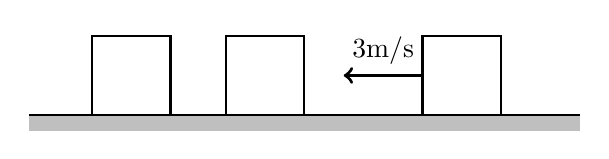
\begin{tikzpicture}
          \fill[gray!50](0,0) rectangle(7,-.2);
          \draw[thick](0,0)--(7,0);
          \draw[thick](.8,0) rectangle(1.8,1);
          \draw[thick](2.5,0) rectangle(3.5,1);
          \draw[thick](5,0) rectangle(6,1);
          \draw[very thick,->](5,.5)--(4,.5) node[midway,above]{\SI{3}{m/s}};
        \end{tikzpicture}
      \end{center}
    }

    \question The speed of the second mass after the collision is
    \label{3masses1}
    \begin{choices}
      \choice zero
      \choice\SI{1.5}{\metre\per\second}
      \choice\SI{3.}{\metre\per\second}
      \choice\SI{6.}{\metre\per\second}
      \choice\SI{9.}{\metre\per\second}
    \end{choices}

  \question The speed of the second and third masses after they collide
    inelastically is
    \label{3masses2}
    \begin{choices}
      \choice zero
      \choice\SI{1.5}{\metre\per\second}
      \choice\SI{3.}{\metre\per\second}
      \choice\SI{6.}{\metre\per\second}
      \choice\SI{9.}{\metre\per\second}
    \end{choices}

    \question A mass traveling in the $+x$ direction collides with a mass at
    rest. Which of the following statements is true?
    \begin{choices}
      \choice After the collision, the two masses will move with parallel
      velocities
      \choice After the collision, the masses will move with anti-parallel
      velocities
      \choice After the collision, the masses will both move along the $x$-axis
      \choice After the collision, the $y$-components of the velocities of the
      two particles will sum to zero.
      \choice None of the above
    \end{choices}
    \vspace{.7in}
    
%    \uplevel{
%      \textbf{Questions \ref{boy1}--\ref{boy2}}
%      
%      A \SI{20}{\kilo\gram} boy runs at a speed of \SI{3.}{\metre\per\second}
%      and jumps onto a \SI{40}{\kilo\gram} sled on frictionless ice that is
%      initially at rest. The boy and the sled then move together for a short
%      time.
%    }
%
%    \question The speed of the boy and sled after he jumps on it is
%    \label{boy1}
%    \begin{choices}
%      \choice\SI{0.5}{\metre\per\second}
%      \choice\SI{0.8}{\metre\per\second}
%      \choice\SI{1.0}{\metre\per\second}
%      \choice\SI{1.5}{\metre\per\second}
%      \choice\SI{2.0}{\metre\per\second}
%    \end{choices}
%    
%    \question While the boy and sled are moving, he jumps off the back of the
%    sled in such a way the boy is at rest, and the sled continues to move
%    forward. The speed of the sled after the boy jumps off is
%    \label{boy2}
%    \begin{choices}
%      \choice\SI{1.5}{\metre\per\second}
%      \choice\SI{2.0}{\metre\per\second}
%      \choice\SI{3.0}{\metre\per\second}
%      \choice\SI{4.5}{\metre\per\second}
%      \choice\SI{6.0}{\metre\per\second}
%    \end{choices}

    \question A \SI{1000}{\kilo\gram} (empty mass) railroad car is rolling
    without friction on a horizontal track at a speed of
    \SI{2.}{\metre\per\second}. Sand is poured into the open top of the car for
    the time interval from $t=0$ to $t=\SI{4.}{\second}$. The mass of the sand
    poured into the car as a function of time is $m(t)=60t^2$. The velocity of
    the car at a time of \SI{4.}{\second} is most nearly
    \cpic{.25}{railroad-car-sand}
    \begin{choices}
      \choice\SI{1}{\metre\per\second}
      \choice\SI{2}{\metre\per\second}
      \choice\SI{3}{\metre\per\second}
      \choice\SI{4}{\metre\per\second}
      \choice\SI{5}{\metre\per\second}
    \end{choices}
    
    \uplevel{
      \textbf{Questions \ref{ramps1}--\ref{ramps2}}
      
      A small block of mass $m$ slides on a horizontal frictionless surface
      toward a ramp of mass $3m$ which is also free to move on the surface. The
      small block slides up to a height $h$ on the ramp with no friction
      (Figure I), then they move together (Figure II), and the small block
      slides back down the ramp to the horizontal surface (Figure III). Both
      the block and the ramp continue to slide on the horizontal surface after
      they separate.
      \cpic{.3}{Figs123}
    }

    \question Which of the following is true regarding the conservation laws
    throughout this process?
    \label{ramps1}
    \begin{choices}
      \choice Kinetic energy is conserved from Figure I to Figure II.
      \choice Momentum is conserved from Figure I to Figure III.
      \choice Kinetic energy is conserved from Figure II to Figure III.
      \choice Potential energy is conserved from Figure I to Figure II.
      \choice Potential energy is conserved from Figure II to Figure III.
    \end{choices}
    \vspace{.7in}
    
    \question Which of the following is a true statement regarding Figure III?
    \label{ramps2}
    \begin{choices}
      \question The small block is moving to the left and the ramp is moving to
      the right.
      \question The small block is moving to the right and the ramp is moving
      to the left.
      \question The small block is moving to the right and the ramp is moving
      to the right.
      \question The small block is moving to the left and the ramp is moving to
      the left.
      \question The small block and the large block are moving with the same
      velocity.
    \end{choices}
    \vspace{.7in}
    \columnbreak
    
    \uplevel{
      \textbf{Questions \ref{remote1}--\ref{remote2}}

      A remote controlled stunt car of mass \SI{800}{\kilo\gram} initially
      moving at \SI{10}{\metre\per\second} is crashed into a rail car of mass
      $m$ that is initially at rest. The cars stick together, and the speed
      $\varv$ of both cars after the collision is given by
      $\varv=\dfrac6{t+1}$.
    }

    \question By considering the fact that the crash occurs at time $t=0$,
    determine the mass $m$ of the rail car.
    \label{remote1}
    \begin{choices}
      \choice\SI{288}{\kilo\gram}
      \choice\SI{445}{\kilo\gram}
      \choice\SI{533}{\kilo\gram}
      \choice\SI{698}{\kilo\gram}
      \choice\SI{800}{\kilo\gram}
    \end{choices}
    
    \question The magnitude of the resisting force acting on the cars as a
    function of time after the collision is
    \label{remote2}
    \begin{choices}
      \choice $\dfrac{6m}{t+1}$
      \choice $6m(t+1)$
      \choice $6m(t+1)^2$
      \choice $\dfrac{6m}{(t+1)^2}$
      \choice $\dfrac{m(t+1)^2}{6}$
    \end{choices}
    \columnbreak
    
    \question A moving object is changing its momentum during a time interval.
    If a graph of momentum vs.\ time is plotted, the net force acting on the
    mass at any time can be determined by finding the
    \begin{choices}
      \choice slope of line tangent to the graph at that time
      \choice area under the graph
      \choice $y$-intercept of the graph
      \choice $x$-intercept of the graph
      \choice change in slope of the graph from beginning to end
    \end{choices}
    \vspace{.7in}
    
%    \question Two masses moving along the coordinates axes as shown collide at
%    the origin and stick to each other. What is the angle $\theta$ that the
%    final velocity that makes with the $x$-axis?
%    \begin{center}
%      \begin{tikzpicture}[scale=.7]
%        \draw(-4,0)--(4,0);
%        \draw(0,-3)--(0,3);
%        \draw[thick,->](-2.5,0)--(-1,0)node[midway,below]{\tiny$\mb{v}_1$};
%        \draw[thick,->](0,-2)--(0,-1)  node[midway,right]{\tiny$\mb{v}_2$};
%        \draw[thick,->](0,0)--(1.3,1.3)node[pos=1,right]{\tiny$\mb{v}_f$};
%        \draw[fill=gray](-2.5,0) circle(.2) node[above]{\tiny$m_1$};
%        \draw[fill=gray](0,-2) circle(.2) node[right]{\tiny$m_2$};
%        \draw[<->] (.75,0) arc(0:45:.75) node[pos=.6,right]{\tiny$\theta$};
%      \end{tikzpicture}
%    \end{center}
%    \begin{choices}
%      \choice $\tan^{-1}(v_2/v_1)$
%      \choice $\tan^{-1}[m_1v_1/(m_1+m_2)]$
%      \choice $\tan^{-1}(m_1v_2/m_2v_1)$
%      \choice $\tan^{-1}(m_2v_2^2/m_1v_1^2)$
%      \choice $\tan^{-1}(m_2v_2/m_1v_1)$
%    \end{choices}
%    \columnbreak
    
    \question A mass $m_1$ initially moving at speed $v_0$ collides with and
    sticks to a spring attached to a second, initially stationary mass $m_2$.
    The two masses continue to move to the right on a frictionless surface as
    the length of the spring oscillates. At the instant that the spring is
    maximally extended, the velocity of the first mass is
    \begin{center}
      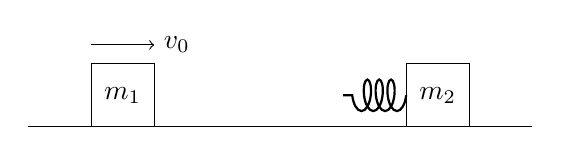
\begin{tikzpicture}[scale=.8]
        \draw[->](1,1.3)--(2,1.3) node[pos=1,right]{$v_0$};
        \draw(0,0)--(8,0);
        \draw(1,0) rectangle (2,1) node[midway]{$m_1$};
        \draw(6,0) rectangle (7,1) node[midway]{$m_2$};
        \draw[thick,
          decoration={aspect=.4,segment length=1.5mm, amplitude=2mm,coil},
          decorate] (6,.5)--(5,.5);
      \end{tikzpicture}
    \end{center}
    \begin{choices}
      \choice $v_0$
      \choice $m_1^2v_0/(m_1+m_2)^2$
      \choice $m_2v_0/m_1$
      \choice $m_1v_0/m_2$
      \choice $m_1v_0/(m_1+m_2)$
    \end{choices}
  \end{questions}
\end{multicols*}
\newpage


\genfreetitle{C}{MOMENTUM, IMPULSE, COLLISIONS, AND CENTER OF MASS}{4}

\genfreedirections

\begin{questions}
  \question A projectile is fired from the edge of a cliff \SI{100}{\metre}
  high with an initial speed of \SI{60}{\metre\per\second} at an angle of
  elevation of \ang{45}.
  \begin{parts}
    \part Write equation for $x(t)$, $y(t)$, $v_x$ and $v_y$. Choose the origin
    of your coordinate system at the particle's original location.
    \part Calculate the location and velocity of the particle at time
    $t=\SI{5}{\second}$.
    
    \uplevel{Suppose the projectile experiences an internal explosion at time
      $t=\SI{4}{\second}$ with an internal force purely in the $y$-direction,
      causing it to break into a \SI{2}{\kilo\gram} and a \SI{1}{\kilo\gram}
      fragment.}
    
    \part If the \SI{2}{\kilo\gram} fragment is \SI{77}{\metre} above the
    height of the cliff at $t=\SI{5}{\second}$, what is the $y$-coordinate of
    the position of the \SI{1}{\kilo\gram} piece?
    
    \part If the speed of the \SI{2}{\kilo\gram} fragment is
    \SI{46}{\metre\per\second} and the fragment is falling at
    $t=\SI{5}{\second}$, what is the $y$-component of the velocity of the
    \SI{1}{\kilo\gram} fragment?
  \end{parts}
  \newpage

  % TAKEN FROM THE 2015 AP PHYSICS C MECHANICS EXAM FREE-RESPONSE QUESTION 2
  \uplevel{
    \cpic{.5}{dart}
  }
  \question A small dart of mass \SI{.020}{\kilo\gram} is launched at an angle
  of \ang{30} above the horizontal with an initial speed of
  \SI{10}{\meter\per\second}. At the moment it reaches the highest point in its
  path and is moving horizontally, it collides with and sticks to a wooden
  block of mass \SI{.10}{\kilo\gram} that is suspended at the end of a massless
  string. The center of mass of the block is \SI{1.2}{\metre} below the pivot
  point of the string. The block and dart then swing up until the string makes
  an angle $\theta$ with the vertical, as shown above. Air resistance is
  negligible.
  \begin{parts}
    \part Determine the speed of the dart just before it strikes the block.
    
    \part Calculate the horizontal distance d between the launching point of
    the dart and a point on the floor directly below the block.
    
    \part Calculate the speed of the block just after the dart strikes.
    
    \part Calculate the angle $\theta$ through which the dart and block on the
    string will rise before coming momentarily to rest.
    
    \part The block then continues to swing as a simple pendulum. Calculate the
    time between when the dart collides with the block and when the block first
    returns to its original position.

    \part In a second experiment, a dart with more mass is launched at the same
    speed and angle. The dart collides with and sticks to the same wooden block.
    \begin{subparts}
      \subpart Would the angle $\theta$ that the dart and block swing to
      increase, decrease, or stay the same? Justify your answer.

      \vspace{.1in}
      \underline{\hspace{.3in}} Increase\hspace{.6in}
      \underline{\hspace{.3in}} Decrease\hspace{.6in}
      \underline{\hspace{.3in}} Stay the same

      \subpart Would the period of oscillation after the collision increase,
      decrease, or stay the same? Justify your answer.

      \vspace{.1in}
      \underline{\hspace{.3in}} Increase\hspace{.6in}
      \underline{\hspace{.3in}} Decrease\hspace{.6in}
      \underline{\hspace{.3in}} Stay the same
    \end{subparts}
  \end{parts}
  \newpage
  
%\item The Ballistic Pendulum. To determine the muzzle speed of a gun, a bullet
%  is shot into a mass $M$ from a string as shown below, causing $M$ to swing
%  upward through a maximum angle of $\theta$.
%  \begin{center}
%    \pic{.4}{ballastic}
%  \end{center}
%  \begin{enumerate}
%  \item What is the speed of $M$ the instant after the bullet lodges in it?
%  \item What is the speed of the bullet before it hits $M$?
%  \item What is the tension in the string at the highest point of the pendulum's
%    swing (when the string makes an angle of $\theta$ with the vertical as
%    shown)?
%  \end{enumerate}
  %  \newpage
  
  \question Two masses are connected by a spring (spring constant $k$) resting
  on a frictionless horizontal surface as shown. The right mass is initially in
  contact with a wall. A brief blow to the left block leaves it with an initial
  velocity $\varv_0$ to the right.
  \begin{parts}
    \part What is the maximum compression of the spring as the left block moves
    to the right?
    
    \uplevel{After the spring is maximally compressed, it eventually moves to
      the left, away from wall. As it moves away from the wall, it continues
      oscillating.
      \begin{center}
        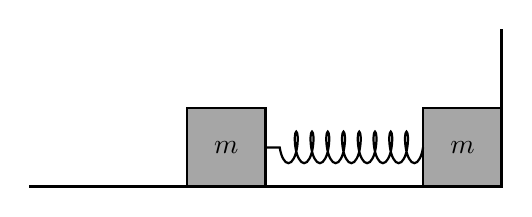
\begin{tikzpicture}
          \draw[thick,fill=gray!70](0,0) rectangle(-1,1) node[midway]{$m$};
          \draw[thick,fill=gray!70](-3,0) rectangle(-4,1) node[midway]{$m$};
          \draw[
            thick,
            decoration={aspect=.3,segment length=2mm, amplitude=2mm, coil},
            decorate] (-1,.5)--(-3,.5);
          \draw[very thick](-6,0)--(0,0)--(0,2);
        \end{tikzpicture}
      \end{center}
    }
    
    \part What is the net momentum of the two masses after they leave the wall?
    
    \part What is the total mechanical energy of the oscillating spring system?
    
    \part What is the relative velocity of the two masses when the spring is
    maximally compressed?
    
    \part What is the maximum compression of the spring after the two masses
    have left the wall? Compare the compression to the maximum compression
    calculated in part (a) and explain any similarities and differences.
  \end{parts}
  \newpage

%\item A stream of glass beads, each with a mass of \SI{.5}{\gram}, comes out of
%  a horizontal tube at $100$ per second. The beads fall a distance of
%  \SI{.5}{\metre} to a balance pan and bounce back to their original height as
%  shown in the figure below. How much mass must be placed in the other pan of
%  the balance to keep the pointer at zero?
%  
%  \cpic{.5}{balance}
%  \newpage

  % TAKEN FROM THE 2011 AP PHYSICS C MECHANICS EXAM FREE-RESPONSE QUESTION 1
  \uplevel{
    \cpic{.25}{projectile}
  }
  \question A projectile is fired horizontally from a launching device, exiting
  with a speed $v_x$. While the projectile is in the launching device, the
  impulse imparted to it is $J_p$, and the average force on it is
  $F_\text{avg}$. Assume the force becomes zero just as the projectile reaches
  the end of the launching device. Express your answers to parts (a) and (b) in
  terms of $v_x$, $J_p$, $F_\text{avg}$, and fundamental constants, as
  appropriate.
  \begin{parts}
    \part Determine an expression for the time required for the projectile to
    travel the length of the launching device.
    
    \part Determine an expression for the mass of the projectile.
    
    \uplevel{The projectile is fired horizontally into a block of wood that is
      clamped to a tabletop so that it cannot move. The projectile travels a
      distance $d$ into the block before it stops. Express all algebraic
      answers to the following in terms of $d$ and the given quantities
      previously indicated, as appropriate.}

    \part Derive an expression for the work done in stopping the projectile.
    
    \part Derive an expression for the average force $F_b$ exerted on the
    projectile as it comes to rest in the block.

    \uplevel{Now a new projectile and block are used, identical to the first
      ones, but the block is not clamped to the table. The projectile is again
      fired into the block of wood and travels a new distance $d_n$ into the
      block while the block slides across the table a short distance $D$.
      Assume the following: the projectile enters the block with speed $v_x$,
      the average force $F_b$ between the projectile and the block has the same
      value as determined in part (d), the average force of friction between
      the table and the block is $f_T$, and the collision is instantaneous so
      the frictional force is negligible during the collision.
    }

    \part Derive an expression for $d_n$ in terms of $d$, $D$, $f_T$, and $F_b$,
    as appropriate.
    
    \part Derive an expression for $d_n$ in terms of $d$, the mass $m$ of the
    projectile, and the mass $M$ of the block.
  \end{parts}

%\item In the billiards shot shown in the figure below, the initial direction of
%  the cue ball is perpendicular to the line joining the centers of the other
%  two balls, which are touching. The cue ball strikes both balls simultaneously.
%  Use the symmetry of the situation along with the appropriate conservation
%  laws to find the final velocities of all three balls.
%  \begin{center}
%    \begin{tikzpicture}[scale=.8]
%      \tikzstyle{balloon1}=[ball color=yellow!60];
%      \tikzstyle{balloon2}=[ball color=green!60!gray];
%      \tikzstyle{balloon3}=[ball color=gray];
%      \draw[dashed](0,-2.4)--(0,2.4);
%      \draw[dashed](0,0)--(-4,0);
%      \shade[balloon2] (0,.4) circle (.4) node{$m$};
%      \shade[balloon1] (0,-.4) circle (.4) node{$m$};
%      \draw[ultra thick,->,blue!60!black](-4,0)--(-2,0)
%      node[pos=1,right]{$\mb{v}_{ci}$};
%      \shade[balloon3] (-4,0) circle (.4) node{$m$};
%    \end{tikzpicture}
%    \hspace{1in}
%    \begin{tikzpicture}[scale=.8]
%      \tikzstyle{balloon1}=[ball color=yellow!60];
%      \tikzstyle{balloon2}=[ball color=green!60!gray];
%      \tikzstyle{balloon3}=[ball color=gray];
%      \draw[dashed](-4,0)--(4,0);
%      \begin{scope}[rotate=25]
%        \draw[dashed](0,0)--(4,0);
%        \draw[ultra thick,->,blue!60!black](4,0)--(5,0)
%        node[right]{$\mb{v}_{1f}$};
%        \shade[balloon2] (4,0) circle (.4) node{$m$};
%      \end{scope}
%      \begin{scope}[rotate=-25]
%        \draw[dashed](0,0)--(4,0);
%        \draw[ultra thick,->,blue!60!black](4,0)--(5,0)
%        node[right]{$\mb{v}_{2f}$};
%        \shade[balloon1] (4,0) circle (.4) node{$m$};
%      \end{scope}
%      \draw(1.5,0) arc(0: 25:1.5) node[pos=.6,right]{$\theta_1$};
%      \draw(1.5,0) arc(0:-25:1.5) node[pos=.6,right]{$\theta_2$};
%      \draw[ultra thick,->,blue!60!black](-2,0)--(-3,0)
%      node[pos=1,left]{$\mb{v}_{cf}$};
%      \shade[balloon3] (-2,0) circle (.4) node{$m$};
%    \end{tikzpicture}
%  \end{center}
%  \vspace{\stretch{1}}  
\end{questions}
\end{document}
